\documentclass{mcmthesis}
\mcmsetup{CTeX = true,   % if use CTeX,set this value as true
        tcn = Competition2, problem = KDDReport, %set team number and problem chosen
        sheet = false, titleinsheet = false, keywordsinsheet = false,
        titlepage = true, abstract = true}%set title page as false can delete the second summary page
\usepackage{ctex}
\usepackage{newtxtext}
\usepackage{amsmath,bm}
\usepackage[T1]{fontenc}
\usepackage[utf8]{inputenc}
\usepackage{authblk}
\usepackage{indentfirst}
\usepackage{graphicx}
\usepackage{listings}
\usepackage{xcolor}
\setlength{\parindent}{2em}
\lstset{
	columns=fixed,       
	frame=none,                                          % 不显示背景边框
	backgroundcolor=\color[RGB]{245,245,244},            % 设定背景颜色
	keywordstyle=\color[RGB]{40,40,255},                 % 设定关键字颜色
	numberstyle=\footnotesize\color{darkgray},           % 设定行号格式
	commentstyle=\it\color[RGB]{0,96,96},                % 设置代码注释的格式
	stringstyle=\rmfamily\slshape\color[RGB]{128,0,0},   % 设置字符串格式
	showstringspaces=false,                              % 不显示字符串中的空格
	language=c++,                                        % 设置语言
}
\title{
	\hspace*{\fill}
	\\ 2021 Spring Data Mining KDD Competition Final Report
	\\ \hspace*{\fill}
	\\ 
\includegraphics[width=0.4\linewidth]{logo.jpg}
	}

\author{
	\Large 计算机科学与技术系 \quad 《数据挖掘》 \ 	兰曼
	\\ Competition2
	\\吴子靖 
	}
\begin{document}

\begin{abstract}
	\par 在本次KDD竞赛系统中,主要目的是通过论文和作者的附属信息,分析出论文和作者之间存在的关系。根据老师提供的改进思路,我们在已有的特征基础上,添加了期刊、会议之间名字的的余弦相似度、论文关键词的tf-idf值作为新的特征。
	\par 撰写的特征函数并不一定需要全选中,精确的选出最佳组合才能让准确率最高,此外分类器的不同也会导致结果的差异,因此我们对单个特征值和不同分类器进行单独测试,根据测试的结果来挑选特征函数组合搭配不同的分类器,同时调参集成,找出出最佳的方案。
	\par 此外,我们针对现在的共作者特征提出了优化方面的猜想:合作频繁到何种程度才应该被选取为共作者?共作者是否有更优秀的权值计算方法?对同一特征函数的不同形式带来的差异提出了讨论:为何用\#\#拼接和分割求均值计算出的准确率差异如此之大?
	
	
	\begin{keywords}
		词向量,语义相似度,去噪处理,ti-idf,pytorch,nltk
	\end{keywords}
\end{abstract}
\maketitle

\tableofcontents 

\section{实验简介}
\subsection {实验环境}
\begin{description}
	\item [\qquad 操作系统] Windows10
	\item [\qquad 实验语言] Python3.9
	\item [\qquad 编辑环境] VsCode
	\item [\qquad 编译环境] Windows PowerShell
	\item [\qquad 安装用包] numpy,sklearn,pandas,pyprind,pytorch,nltk,re
\end{description}
\subsection{实验系统}
\par KDD基准系统:由一系列数据文件和代码文件组成,数据文件包括源数据文件、通过代码生成的辅助文件和训练测试文件。
\par 源数据文件包括Author.csv,Paper.csv,PaperAuthor.csv,Conference.csv and Journal.csv. 
\begin{itemize}
	\item Author.csv描述了作者的信息,包括编号,名称与隶属单位
	\item Paper.csv描述了论文的信息,包括编号,标题,年份,会议/期刊以及论文关键字
	\item PaperAuthor.csv包含了若干个(PaperId,AuthorId)的元组,表面了该作者写过该论文
	\item Conference.csv描述了会议的详细信息
	\item Journal.csv描述了期刊的额详细信息
\end{itemize}
\par 辅助文件和训练测试文件的内容我们将在后文进行阐释,对于以上五项文件,系统中明确说明的是对于Author.csv,Paper.csv和PaperAuthor.csv存在噪音:除了某些附属信息项存在缺失之外,还存在作者多名,论文多源发表和PaperAuthor.csv本身存在错误的情况。
\subsection{数据规模}
\begin{center}
	\begin{tabular}{cc}
		\hline
		数据集          &   数据规模        \\
		\hline
		Train.csv       &   11263  \\
		Valid.csv       &   2347  \\
		Train.csv       &   1300  \\
		Author.csv      &   5000  \\
		Paper.csv       &   61w  \\
		PaperAuthor.csv &   104w  \\
		Journal.csv     &   15000  \\
		Conference.csv  &   4500  \\
		\hline
	\end{tabular}
\end{center}
\section{实验目的}
	\par 实验的直观目的为:对于给定的(AuthorId,PaperId),判断该作者是否写了该篇论文。有趣的是已经存在PaperAuthor.csv文件描述了作者和论文之间的关系,但该文件又存在噪音,因此如何看待该文件的存在成了解决问题的关键。
	\par 重新审视五个数据文件,除了Id属性之外,每个文件都存在着其他附属信息,如单位,关键词,姓名,标题等。实验的目的便是通过给予的附属信息,生成分类特征,然后通过分类器算法标注给定的论文-作者对。
\section{实验内容}
	\subsection{运行系统}
	\par 在拿到KDD系统之后,首先检测该系统能够正常执行,因此对于所有包含main函数的代码,都在Windows PowerShell中执行python pyfile.py来检验是否正常,在以下几个文件中,出现了一些小问题:
	\begin{description}
		\item [\qquad \quad config.py] CWD ="...$\backslash$KDD\_Benchmark"需加上字母r修改为CWD = r"...$\backslash$KDD\_Benchmark",原因是在windows系统中读取文件路径可以使用$\backslash$,但$\backslash$在python的字符串中有转义的含义,因此加上关键字r使其不被解读为转义字符。
		\item [\qquad \quad trainer.py] json.load(open(file,"r"),encoding="utf-8")需修改为json.load(open(file,"r",encoding="utf-8")),也许是python版本差异导致写法的不同。
		\item [\qquad \quad coauthor.py] \hspace*{\fill}
			\begin{itemize}
				\item print output 修改为 print(output),前者是python2的写法
				\item reload(sys)要在import importlib之后修改为importlib.reload(sys),前者也是python2的写法
			\end{itemize}
		\item [\qquad \quad stringDistance.py] 同coauthor.py,将一些python2的写法修改为python3
		\item [\qquad \quad util.py] 将with open(in\_file)修改为 with open(in\_file,"r","utf-8")来指定编码方式
	\end{description}
	
	\par 修改完上述内容之后,执行python train.py文件,成功得到运行结果

	\begin{figure}[h]
		\centering
		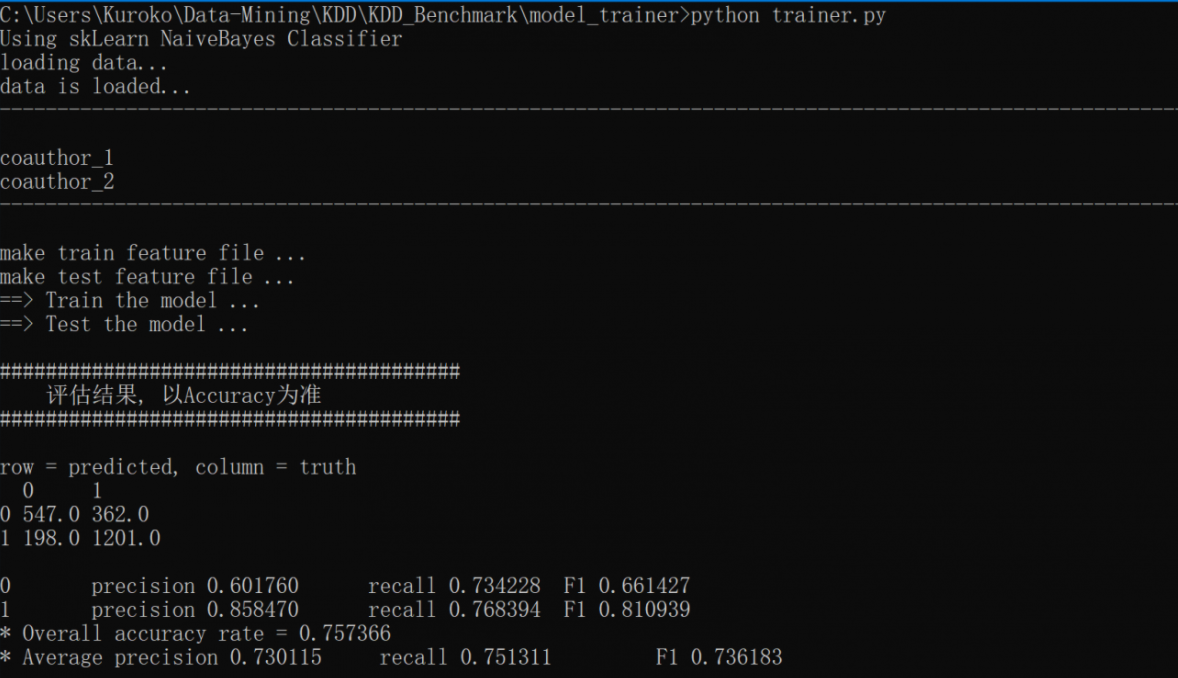
\includegraphics[width=0.8\linewidth]{p1.png}
		\caption{首次运行系统}
		\label{fig:p1}
	\end{figure}
	\subsection{辅助测试}
	\par 在阅读问数据文件的描述内容之后,对于各个文件的噪音有些许疑问,因此分别撰写了一些辅助文件来进行测试:
		\subsubsection{Author.csv}
		\par 在该文件中提到"相同的作者可能在数据集中出现多次,因为作者在不同会议/期刊上发表论文的名字可能有多个版本"。那么同一个作者的两中呈现形式在该文件中的Id字段是否相同?如果是,那么可以做一个合并工作来简化系统;如果不是,那么又改如何利用Name信息。为了解决该问题,撰写了辅助文件TestAuthor.cpp(初期希望用cpp因为执行效率更高,但后面的文件中因为字段本身也存在逗号,尽管有引号标识,但是需要用状态机来读取,因此后续辅助文件的语言又换回了Python),代码流程为:
		\begin{itemize}
			\item 获取当前的文件目录,返回文件路径
			\item 读取Author.csv到StringStream
			\item 以Id字段为key,以vector<Name>为val,构建哈希表
			\item 将每一项存储到哈希表
			\item 查看是否存在某个key的vetor容量大于1
		\end{itemize}
		\par 最终的结果为并不存在这样的项,也就是说,J.Doe和Jane Doe所拥有的Id值也是不同的,那么通过Name找Id的想法是不可行的。只能计算不同项之间Name的语义相似度。
		{\setmainfont{Courier New Bold}               
			\begin{lstlisting}
	//Code Listing 1: TestAuthor.cpp
	# include <iostream>
	# include <fstream>
	# include <cstdlib>
	# include <sstream>
	# include <unordered_map>
	# include <vector>
	using namespace std;
	
	//得到系统路径
	string getDataPath(string path) 
	{
		stringstream ss;
		string WD = _pgmptr,s; //to get the present directory
		int count = 0;
		while(WD.find("\\") != string::npos) 
		{
			WD.replace(WD.find("\\"),1," ");
			count++;
		}
		ss<<WD;
		WD.clear();
		for(int i = 0;i < count-1;i++) 
		{
			ss>>s;
			WD += s+"\\";
		}
		WD += path;
		return WD;
	}
	
	
	int main(void)
	{
		stringstream ss;
		string line,key,value,tmp;
		# 读取数据文件
		string dataPath = getDataPath("data\\dataset\\Author.csv");
		ifstream inStream(dataPath,ios::in);
		unordered_map<int,vector<string>> dict;
		getline(inStream,line);
		while(getline(inStream,line))
		{
			key = line.substr(0,line.find(","));
			line = line.substr(line.find(",")+1);
			value = line.substr(0,line.find(","));
			# 用Id作为key值,用Name作为val值
			dict[stoi(key)].push_back(value);
		}
		# 检测是否有哪个Id包含多个Name
		for(auto it = dict.begin();it != dict.end();it++)
		{
			if(it->second.size() > 1)
			{
				cout<<it->first<<":{";
					for(int i = 0;i < it->second.size();i++)
					cout<<it->second[i]<<(i==it->second.size()-1?"}\n":",");
			}
		}
		return 0;
	}
			\end{lstlisting}
		}
\lstset{
	columns=fixed,       
	frame=none,                                          % 不显示背景边框
	backgroundcolor=\color[RGB]{245,245,244},            % 设定背景颜色
	keywordstyle=\color[RGB]{40,40,255},                 % 设定关键字颜色
	numberstyle=\footnotesize\color{darkgray},           % 设定行号格式
	commentstyle=\it\color[RGB]{0,96,96},                % 设置代码注释的格式
	stringstyle=\rmfamily\slshape\color[RGB]{128,0,0},   % 设置字符串格式
	showstringspaces=false,                              % 不显示字符串中的空格
	language=Python,                                     % 设置语言
}
		\subsubsection{Paper.csv}
		\par 相同的问题也在Paper.csv中进行了检验:即一个论文的多个副本在不同的平台上的其他信息是否是相同或相似的?如拥有相同或近似的标题,关键词和年份?为了解决该疑问,撰写了辅助文件TestPaper.py,代码的流程很朴素:首先将Paper.csv读取到DataFrame中,然后分别以Title,Year和Keywords为关键字进行字典序排序,然后重新索引之后写入新文件中,然后观察相邻项之间是否有相同或极其相似的情况。尽管字典序排序会丢失大量语义信息,但是对于完全相同或仅有个别关键字不同的组,还是可以发掘出的。Year的结果意义不大,Keywords因为存在太多空缺,也没什么意义,这里给出以Title的执行结果文件的部分截图:
			\begin{figure}[h]
			\centering
			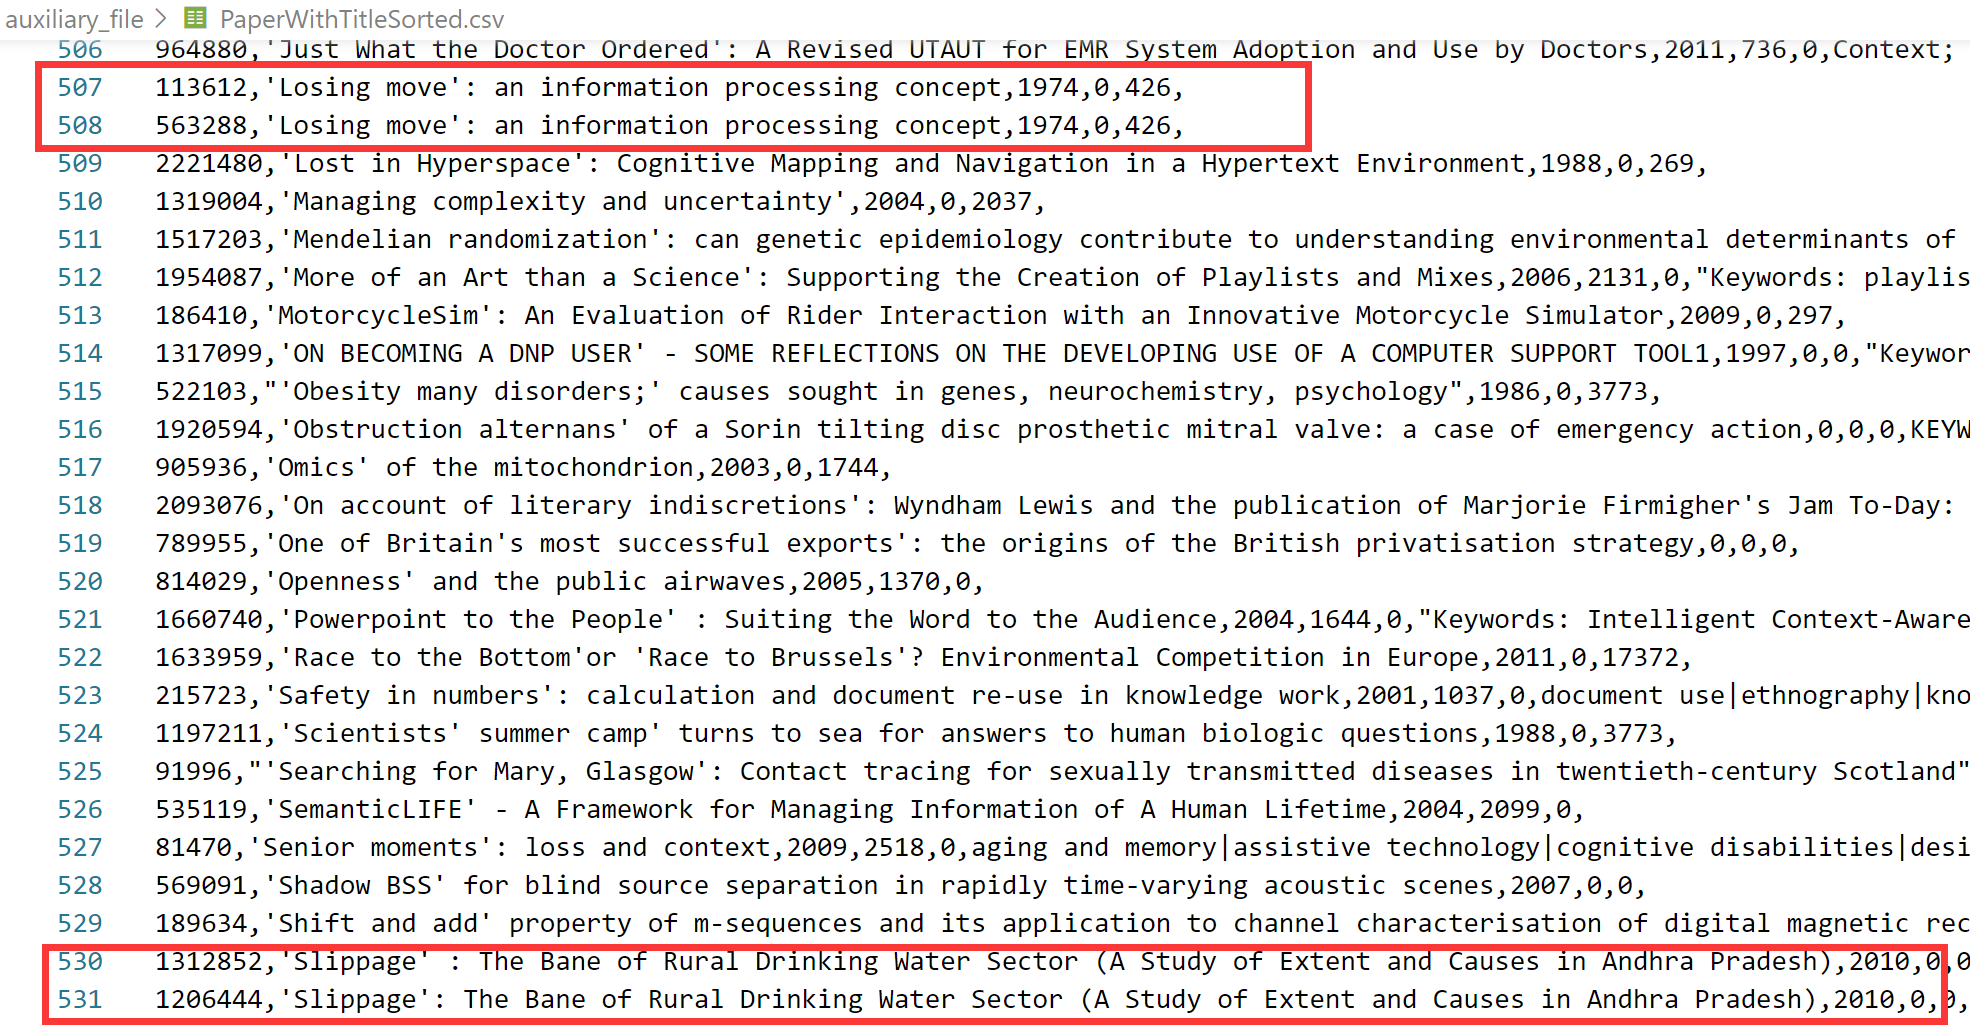
\includegraphics[width=0.8\linewidth]{p2.png}
			\caption{PaperWithTitleSorted.csv部分截图}
			\label{fig:p2}
			\end{figure}
		\par 可以发现,尽管是以最朴素的方式寻找相邻的项,也可以找到一些完全相同的或近似的结果,那么如果用语义分析出的相似度来进行分组,必然存在更多的心意可以挖掘,对于上图中的113612,563288我们便可以直接认定他们为同一篇论文,于是可以将他们的关键词进行相互补充,提高后续特征值的精确度。对于标题近似的项,还可以将他们的标题词汇相互补充,这些部分内容会在后文进行说明。相比于Author.csv,Paper.csv的测试结果还是提供了一些信息的。
	
		{\setmainfont{Courier New Bold}              
			\begin{lstlisting}
	#Code Listing 2: TestPaper.py
	#encoding: utf-8
	import os
	import sys
	import importlib
	import numpy as np
	from pandas import Series, DataFrame
	import pandas as pd
	importlib.reload(sys)
	sys.path.append("../")
	import config
	if __name__ == '__main__':
		paper_file_path = os.path.join(config.DATASET_PATH,"Paper.csv")
		data = pd.read_csv(paper_file_path, encoding='utf-8')
		data = data.sort_values(by = "Title")
		data = data.reset_index(drop = True)
		data.to_csv("PaperWithTitleSorted.csv",index=False)
			\end{lstlisting}
		}
	\subsection{源码简述}
		\par 实验系统中涉及数十个代码文件,为了更好的理解系统的工作原理,首先进行源代码的阅读并注释。其中有许多代码内容为变量名的定义、类的定义、数据集的加载和函数的调用,对于此类代码,这里便不做赘述。对于confusion\_matrix.py,内容复杂且与实验核心无关,因此也不做阐述。而对于coauthor.py,stringDistance.py,util.py这类与特征文件相关的,我们将对其流程和关键代码进行简短的描述:
		\subsubsection{coauthor.py}
		\par 该文件是生成数据文件coauthor.json的代码。其算法为:对于PaperAuthor.csv中的内容,如果出现了(Pid,Aid1)和(Pid,Aid2)那么便认为Aid1和Aid2合作完成了Pid这篇论文,因此首先建立一个字典:其key值为Pid,val值为list[Aid],将每篇论文的全部作者以列表的形式存储。然后将(Aid1,Ai2d)看成图的一条有权无向边,当在某个list中同时出现了Aid1与Aid2时,无向边的权重+1,也就是代码中的:
			\begin{description}
			\item [\qquad \quad] dict\_author\_to\_coauthor[authors[i]][authors[j]] += 1
			\item [\qquad \quad] dict\_author\_to\_coauthor[authors[j]][authors[i]] += 1
			\end{description}
		最后通过调用Counter的most\_common函数,只将最频繁出现的k个值写入字典中,转换成authorId:{coauthorId1:c1,coauthorId2:c2...}的形式并写入json文件中。可以通过修改代码中k的值来重设文件,实际执行的过程中发现,由于PaperAuthor.csv文件的行数高达100w,令n = 文件行数,m = 文件中的Paper种类数,k = 文件中的Author种类数, 于是代码第一步合并的复杂度为$O(n)$,第二步加权的复杂度为$O(m^2)$,第三步统计的复杂度为$O(k^3\log(k))$,整个代码的复杂度并不算低,导致运行时间需要几十分钟。

		\subsubsection{stringDistance.py}
		\par 该文件是生成数据文件paperIdAuthorId\_to\_name\_and\_affiliation.json的代码,其内容同样来自PaperAuthror.csv中。主要目的是去除该文件的噪音之一,该噪音没有在文件描述中说到,但在该代码的注释中提到:"PaperAuthor.csv文件包含噪音的,同一个(authorid,paperid)可能出现多次"。代码的流程是以(authorId,paperId)为键值,以其他附属信息为value,用字典进行合并,其中因为(authorId,paperId)没有hash的方式,因此写入字符串"authorId|paperId"来进行hash。最后再用"\#\#"进行拼接,写入json文件。
		\par 不难发现,此类噪音的去除方式与上文3.2.2 Paper.csv小节的阐述近似,我们曾说道"对于Title完全一致的两个项,可以考虑将他们的附属信息进行合并。而对于不相同的项,可以通过语义相似度的计算进行判定,如果两个项的相似度足够大,可以认定他们为同一项,然后进行附属信息的合并"。在AuthorPaper.csv中,信息中的噪声是显式的,即明确说明了会有(PaperId,AuthorId)完全一样的若干个项,而在Paper.csv与Author.csv当中,重复项是隐式的,同一个作者的多种形式仅在Name和Affiliation上有可能有关联,且Affiliation还有可能为空。论文同理,同一篇论文多次出现的Title和Keyword有可能有关联,且Keyword有可能为空。我们无法类比stringDistance.py中的处理方法,因为此类合并除了错误的记录以外,是保证正确的合并。而通过语义计算出的结果进行合并是有一定风险的,该问题的还涉及阈值、计算方法、合并方式等问题,将在问题讨论部分进行探讨。
		
		\subsubsection{util.py}
		\par 小工具类文件,包括了文件读写类的函数和特征相关类的函数,我们仅介绍与特征相关的函数。
		\hspace*{\fill} \\
		\begin{tabular}{l}
			\hline
			Function 1: get\_feature\_by\_list \\
			输入: 列表,内部元素类型为int or float \\
			输出: 一个特征类 \\
			假设输入的list L = [A,B,C,D,E....N], len(L) = n, 那么首先构造出字典: feat\_dict = {1:A,2:B,...n:N} \\
			然后以此为参数构造一个Feature类:Feature.feat\_string = "1:A 2:B 3:C ... n:N" \\
			\hline
			def get\_feature\_by\_list(list): \\
			\qquad feat\_dict = {} \\
			\qquad for index, item in enumerate(list): \\
			\qquad \qquad if item != 0: \\
			\qquad \qquad \qquad feat\_dict[index+1] = item \\
			\qquad return Feature("", len(list), feat\_dict) \\ 
			\hline
		\end{tabular}
		
		\par 该函数是添加新的特征函数的接口,将新写好的特征函数名加入到train.py的feature\_function\_list中,并在特征函数中将计算出的特征值按照list的形式传入该函数,那么就能生成出对应的特征类,最终加入到特征文件当中。
		\hspace*{\fill} \\
		\begin{tabular}{l}
			\hline
			Function 2: mergeFeatures \\
			输入: 列表,内部元素类型为Feature类 \\
			输出: 一个特征类 \\
			\hline
			def mergeFeatures(feature\_list, name = ""): \\
			\qquad dimension = 0 \\
			\qquad feat\_string = "" \\
			
			\qquad \# 枚举每一个Feature对象 \\
			\qquad for feature in feature\_list: \\
			\qquad \qquad if dimension == 0:\#第一个 \\
			\qquad \qquad \qquad feat\_string = feature.feat\_string \#赋值特征 \\
			\qquad \qquad else: \\
			\qquad \qquad \qquad if feature.feat\_string != "": \\
			\qquad \qquad \qquad \qquad \#修改当前feature的index \\
			\qquad \qquad \qquad \qquad temp = "" \\
			\qquad \qquad \qquad \qquad for item in feature.feat\_string.split(" "): \\
			\qquad \qquad \qquad \qquad \qquad \# 取原下标和特征值 \\
			\qquad \qquad \qquad \qquad \qquad index, value = item.split(":") \\
			\qquad \qquad \qquad \qquad \qquad \# 构造新索引 \\
			\qquad \qquad \qquad \qquad \qquad temp += " \%d:\%s" \% (int(index)+dimension, value) \\
			\qquad \qquad \qquad \qquad feat\_string += temp \# 合并特征值 \\
			\qquad \qquad dimension += feature.dimension \# 加上维度值 \\
			\qquad \# 最后构造一个特征类,将合并的特征值去除首尾空格后(strip)赋值 \\
			\qquad merged\_feature = Feature(name, dimension, \{\}) \\
			\qquad merged\_feature.feat\_string = feat\_string.strip() \\
			\qquad return merged\_feature \\
			\hline
		\end{tabular}
		\par 首先关注get\_feature\_by\_list函数,该函数中有 if item != 0:这一条语句,说明了不会记录值为0的特征,但index不会因此停滞,即[1,0,6,7]的输入生成的Feature特征类的feat\_string = "1:1 3:6 4:7",2:0不会记录,但6的index值仍为2,不会前移。mergeFeatures的作用是将多个特征类合并为一个,其中index要递增,此时显现出dimension的作用 。考虑列表[5,7,9,0]生成的特征类,feat\_string = "1:5 2:7 3:9",但实际上是存在第四维的,直接通过feat\_string无法获取,需要用dimension = len(list)来记录维数。合并的方式是通过split函数还原成int值,然后通过dimension与index相加的方式重构字符串,对于上述两个特征类,合并出来的结果是feat\_string = "1:1 3:6 4:7 5:5 6:7 7:9",dimension = 8,该函数应用于每一项,具体来说对于每一个(PaperId,AuthorId),都会调用全部的特征函数生成多个特征值,但列名/索引均是从1开始的,因此需要改函数的帮助进行索引的重设和字符串的合并。
		
		\par 最后是关于example写入文件的函数,对于.feature文件,写入的格式为
		$$ \rm tag \quad key_1:val_1 \quad key_2:val_2 \quad ... \quad key_n:val_n \quad \# \quad paperId \quad authorId $$
		对于.arff文件,在网络上搜索了他的定义:arff:Attribute-Relation File Format。arff是一个ASCII文本文件,记录了一些共享属性的实例。
		此类格式的文件主要由两个部分构成,头部定义和数据区。头部定义包含了关系名称(relation name),一些属性(attributes)和对应的类型。数据区则定义了特征值和类标。
		\hspace*{\fill} \\
		\begin{tabular}{ll}
			\hline
			Function 3: write\_example\_list\_to\_arff\_file (部分) & \\
			out\_lines.append("@relation kdd")  & arff关系名称命名为kdd \\
			out\_lines.append("@attribute attribution\%d numeric" \% (i+1)) & arff属性名称 属性类型为numeric数值类型 \\
			out\_lines.append("@attribute class {0, 1}") & arff类标取值类型限定为{0,1} \\
			out\_lines.append("@data")  & arff数据区域字段开始 \\
			out\_lines.append("\%s,\%s" \% (feature, target)) & 写入特征值,类标 \\
			\hline
		\end{tabular}
		\par make\_feature\_file.py尽管与特征文件相关,但是其内容均为调用util.py的函数和example的构造函数,因此就无需赘述。
	\subsection{已有特征}
	\subsubsection{coauthor}
		\par 在3.3.1节中介绍了coauthor.json文件的生成方式,该文件正是服务于coauthor特征函数。对于该特征的设计思路,我们的理解为:对于作者A,已知他经常与$\rm P_1,P_2,P_3,P_k$进行合作,现在有一篇论文M,那么如果$\rm P_1$到$\rm P_k$全部参与了这次创作,A显然也极有可能参与。而在非理想的情况下,这k个人当中越多人参与,A参与的可能性就越高。该特征最显著的两个参数是k和weight:即最合作频繁到什么程度的作者可以参与运算,参与这次创作的作者所占权重为多少。我们将该问题的讨论放在"5.问题讨论"中,现在假定k = 10,而权重的计算方法为老师提供的两种:
		\begin{itemize}
			\item 人人平等,所有人的权重均为1
			\item 权重 = 合作次数
		\end{itemize}
		\par 直观上看,方案2显然更加合理,因为和你合作100次的人参与了此次创作的意义显然不同于仅和你合作过1次的,但是考虑这样一种情况,A参与了一个专家小组,里面共20人,还有一个挚友B。专家小组发表了100篇论文,每篇论文都会有这20个人当中的一半,那么A参与的论文数 = C(19,9)/C(20,10)*100 = 50篇,而每个人和A合作的期望是C(18,8)/C(20,10)*100 = 23次,A和挚友B两人一起发表过5篇文章。假设现在已知一篇论文M,专家小组有一个人C和A合作了23次,B和A只合作了5次,若C参与了M的创作,那么A参与创作的概率是C(18,8)/C(19,9)=0.47,但是B如果参与了M的创作,那么尽管无法用概率衡量,但是也不一定亚于0.47,至少不会到23:5的概率比,因此考虑现实因素,方案1未必逊色于方案2。最终结果依赖看数据集的特性,在未知的情况下,我们可以将两种方式均加入特征的计算。
	\subsubsection{stringDistance}
		\par 再关注stringDistance的计算方式,考虑PaperAuthor.csv不存在任何噪声的情况,对于任何输入的论文作者对,可直接通过查询其是否存在PaperAuthor.csv中来进行类别的标注。
		而现在对于PaperAuthor文件,其内部是有若干条错误记录的。换句话说,每条记录都有一定概率正确,一定概率错误,我们称正确的概率为可信度。stringDistance的工作等同于计算可信度。为了更好的阐述后文,我们先命名一些参数,假定输入的作者id为Aid,输入的论文id为Pid,于是从Author.csv文件中可以查询到Aid对应的Name与Affiliation。而在PaperAuthor.csv当中,也出现了若干个(Pid,Aid,Name,Affiliation)的四元组,但Pid或Aid是可能出现记录错误,对于正确的记录而言,同一个Aid在Author文件中出现的Name和Affiliation应该与PaperAuthor文件中的Name和Affiliation相同或近似。所以如果二者之间的语义/文本的近似程度决定了可信度,而可信度越高,标签就越有可能是positive的,于是最后直接将计算出来的相似度充当特征值。
		\par 老师为相似度的计算提供了三种算法,均是字符串距离的算法而非语义相似度。事实上,对于Name和Affiliation属性而言,字符串距离在时间和正确率上的效果都要优于语义相似度,这是因为一个人的多种姓名往往都是缩写全称分别,他们在文本上近似,但若转换成词向量,差异反而很大。附属单位往往也只是缩写、缺省、倒装的差异,亦或者是完全不同,因为观察数据可以发现,一个人往往隶属于几个完全无关联的单位。此外,姓名和隶属单位含有大量专有名词,在词性还原的工作上也难以进行。综合上述情况,字符串距离是比较理想且高效的方法。
		\par 对于提供的两种计算方式,直感上是方法2较好,因为分割之后排除了\#\#带来的影响,但同样,评判还是需要通过实践来检验。
	\subsection{新增特征}
		\subsubsection{Conference\&Journal}
			对于该部分,我么采用了老师提供的方案:考虑作者aid之前发表的论文的journal和conference,与当前的论文pid的journal和
			conference之间的相似度,作为特征。相似度的计算方式我们调用了torch库中的Embedding方法,分词还原等操作调用了nltk库。
			首先介绍我们为该特征撰写的若干个函数:
			\par 函数1: get\_origin\_word\_from\_sentence,意为得到一个句子的全部单词,且单词均是经过了词性还原的。整个函数的流程参照了《自然语言处理》课程的"文本处理基础"。
			\begin{description}
				\item [\qquad 语句分词]调用nltk.tokenize.word\_tokenize方法
				\item [\qquad 标准处理]用正则表达式只保留数字和字母,然后调用nltk.corpus.stopwords方法来去停用词
				\item [\qquad 词干提取]调用nltk.stem.porter.PorterStemmer().stem方法
				\item [\qquad 词性标准]调用nltk.pos\_tag方法
				\item [\qquad 词性还原]调用nltk.stem.WordNetLemmatizer().lemmatize方法
			\end{description}
			函数的输入参数是单个字符串,返回一个列表,列表中的每个元素是单词字符串,该函数应用于Conference和Journal的FullName处理,同时也用于构建词典,是计算本轮特征值的重要成员。
			{\setmainfont{Courier New Bold}              
				\begin{lstlisting}
	#Code Listing 3: my_feature.py @get_origin_word_from_sentence
	def get_origin_word_from_sentence(sentence):
		pattren = re.compile("[^a-zA-Z0-9\n]") #数字字母的正则匹配
	
		#分词    
		Tokenization = tk.word_tokenize(sentence) 
	
		#标准化
		Normallization = []
		for word in Tokenization:
			# 将所有非数字字母字符全部转换为空格,并统一小写化
			word = re.sub(pattren," ",word).lower()
			word = tk.word_tokenize(word) #再次分词
			#去停用词
			word = [w for w in word if (w not in stopwords.words("english"))]
			Normallization += word
	
		#词干提取
		Stemming = []
		for word in Normallization:
			pt_stem = nltk.stem.porter.PorterStemmer().stem(word)
			Stemming.append(word)
	
		#词性标注
		word_pos = nltk.pos_tag(Stemming)
		
		#词性还原
		Lemmatization = []
		lemmatizer = ns.WordNetLemmatizer()
		for item in word_pos:
			word = item[0]
			tag = item[1][0].lower()
			if tag == 'j':
				tag = 'a'
			elif tag == 'r' or tag == 'v':
				tag = tag
			else:
				tag = 'n'
			Lemmatization.append(lemmatizer.lemmatize(word,tag))
		return Lemmatization
				\end{lstlisting}
			}
			\par 函数2: Make\_dictionary,词典的制作,实际上就是为后续词向量构建词典。函数的流程为:
			\begin{itemize}
				\item 读入Journal.csv/Conference.csv文件
				\item 提取每一行的FullName参数值
				\item 调用上文的get\_origin\_word\_from\_sentence函数,将FullName分成若干个单词
				\item 将所有单词插入集合中
				\item 最终得到的集合包含了文件处理后的全部单词
				\item 将集合的内容写入txt文件,在计算特征函数的时候读取
			\end{itemize}
			函数的输入是读取的文件路径和生成词典的文件路径,配合下文的Read\_dict\_from\_txt函数使用。
			{\setmainfont{Courier New Bold}              
				\begin{lstlisting}
	#Code Listing 3: my_feature.py @Make_dictionary
	def Make_dictionary(source_file,to_file):
		source = pd.read_csv(source_file)
		lines = len(source)
		word_set = set()  #集合去重

		for i in range(lines):
			name = source["FullName"][i]
			if name == "nan": #数据缺失
				name = ""
			words = get_origin_word_from_sentence(str(name))
			for word in words:
				word_set.add(word)

		with open(to_file, 'w', encoding = "utf-8") as fout:
			for word in word_set:
				fout.write(word+"\n")
				\end{lstlisting}
			}
			\par 函数3: Read\_dict\_from\_txt,词典的读取,需要注意的是读入的容器不再是集合,而是字典。字典的key值为单词本身,val值为单词所在的行号。这是因为要用该字典作为Embedding方法的参数,要求每个单词有一个索引值,因此用行号来充当。
			{\setmainfont{Courier New Bold}              
				\begin{lstlisting}
	#Code Listing 3: my_feature.py @Read_dict_from_txt
	def Read_dict_from_txt(source_file):
		dict = {}
		index = 0
		with open(source_file, 'r', encoding = "utf-8") as fin:
			content = fin.readlines()
			for i in range(len(content)):
				dict[content[i][:-1]] = i#去除换行符
		return dict
				\end{lstlisting}
			}
			\par 函数4: cosine\_similarity,计算两个词向量的余弦相似度
			{\setmainfont{Courier New Bold}              
				\begin{lstlisting}
	#Code Listing 3: my_feature.py @cosine_similarity
	def cosine_similarity(vector_a,vector_b):
		vector_a = vector_a.detach().numpy()[0]
		vector_b = vector_b.detach().numpy()[0]
		dimension = len(vector_a)
		sum = 0
		mod_a = 0
		mod_b = 0
		for i in range(dimension):
			sum += vector_a[i]*vector_b[i]
			mod_a += vector_a[i]**2
			mod_b += vector_b[i]**2
		return sum/(numpy.sqrt(mod_a*mod_b))
				\end{lstlisting}
			}
			
			\par 函数5: journal\_similarity,特征函数,与之对应还有一个conference\_similarity函数,由于两个文件构造完全一致,因此两个函数除了几个参数名一样以外,其余完全一致,所以这里仅展示journal\_similiaryity的代码。函数的流程为:
			\begin{itemize}
				\item 调用Read\_dict\_from\_txt读取Make\_dictionary生成的词典
				\item 以字典为参数,调用torch.nn.Embedding方法,其中词向量维度设置了200维
				\item 获取aid写过的全部论文all\_papers
				\item 获取pid对应的journalId,再通过journalId获取FullName
				\item 调用get\_origin\_word\_from\_sentence解析FullName
				\item 对FullName中的每个word调用torch.LongTensor方法获取词向量,并转换为张量
				\item 加权除以单词个数,得到最终FullName的向量
				\item 对于all\_papers中的每篇论文,采取相同的流程
				\item 调用cosine\_similarity计算pid与all\_papers中的每篇论文的余弦相似度
				\item 除以all\_papers的论文数量得到平均值,作为最终特征值
			\end{itemize}
			{\setmainfont{Courier New Bold}              
				\begin{lstlisting}
#Code Listing 4: feature_fuctions.py @journal_similarity
def journal_similarity(AuthorIdPaperId, dict_coauthor, dict_paperIdAuthorId_to_name_aff, 
					   PaperAuthor, Author, Paper, Journal, Conference):
	# 从类成员中提取作者id与论文id
	authorId = AuthorIdPaperId.authorId
	paperId = AuthorIdPaperId.paperId
	
	# 搜索该作者以前写过的全部论文
	all_papers = list(map(str, list(PaperAuthor[PaperAuthor["AuthorId"] == int(authorId)]["PaperId"].values)))
	
	# 搜索输入论文对应的期刊id
	journalId = list(map(str, list(Paper[Paper["Id"] == int(paperId)]["JournalId"].values)))
	if len(journalId) == 0:
		return util.get_feature_by_list([0])
	
	# 搜索该会议id对应的FullName
	fullName = list(map(str, list(Journal[Journal["Id"] == int(journalId[0])]["FullName"].values)))
	if len(fullName) == 0:
		return util.get_feature_by_list([0])
	
	# 读取字典
	journal_dict = Read_dict_from_txt(config.JOURNAL_DICT)
	
	# 词向量维度
	dimension = 200

	# 初始化embeds
	embeds = torch.nn.Embedding(len(journal_dict),dimension)

	word_vector_x = torch.zeros(1,dimension)
	fullName = get_origin_word_from_sentence(fullName[0])
	for word in fullName:
		v = embeds(torch.LongTensor([journal_dict[word]]))
		word_vector_x.add_(v)
	word_vector_x /= len(fullName)

	result = 0
	cnt = 0
	for pid in all_papers:
		jid = list(map(str, list(Paper[Paper["Id"] == int(pid)]["JournalId"].values)))
		if len(jid) == 0:
			continue

		name = list(map(str, list(Journal[Journal["Id"] == int(jid[0])]["FullName"].values)))
		if len(name) == 0:
			continue
		cnt += 1
		word_vector_y = torch.zeros(1,dimension)
		name = get_origin_word_from_sentence(name[0])
		for word in name:
			v = embeds(torch.LongTensor([journal_dict[word]]))
			word_vector_y.add_(v)
		word_vector_y /= len(name)
		cs = cosine_similarity(word_vector_x,word_vector_y)
		if abs(cs) > 0.05: #阈值
			result += cs
	result /= cnt
	return util.get_feature_by_list([result])
				\end{lstlisting}
			}
			\par 在实际测试的过程中,该函数的经历了一系列改善:
			\begin{description}
				\item [\qquad \quad 浮动太大] 我们任选了两项FullName作为参数,首先设置了20的词向量维数,然后循环100次,每一次重新构建Embeddings,然后打印他们的余弦相似度。出乎意料的是,结果最小可以到0.001,最大可以到0.93,100次的测试结果更像是rand出来的。后来了解到,Embeddings本身就是一种随机构建的方案,但是会在构建的过程中不断调整,最终趋向于正态分布。而20维的维度数过低,加上词典本身规模也不大,导致了结果就是一种随机。既然无法修改词典的数量级,我们开始不断增加词向量的维度。欣慰的是,随着词向量的维度不断增大,结果也不断趋于稳定。对于x = "IEEE Transactions on Dependable and Secure Computing",y = "IEEE Transactions on Evolutionary Computation",在维度达到200的时候,他们的相似度稳定在了0.7-0.85之间,尽管区间还是有一定影响,但我们认为已经是比较理想的结果。我们在200的基础上继续增大,但是至此常数级的改动已经对结果的影响很小了,即使增加到1000维,结果的浮动区间还是达到了0.1的长度。相反,特征的训练时间已经从200维的20分钟变成一个小时了。于是我们最终采用了200维的方案。
				\item [\qquad \quad 阈值选择] 即使两个毫无关联的句子,他们的语义相似度也可能有一定比重,对于计算结果为0.003,0.05乃至0.1我们均可以认为就是没有关系的,但是也会一定程度的影响均值,于是我们需要敲定一个阈值,筛选掉过小的值来保护真正有价值的信息。我们通过反复测试,最终使用了0.05作为最终阈值。
				\item [\qquad \quad 方案选择] 与样例特征类似,我们同样为会议/期刊特征提供了两种形式的特征函数。因为在实际操作中发现,绝大多数样例要么发表在期刊,要么发表在会议,于是我们撰写了函数来检验该想法,最终发现只要一篇paper同时发表在了会议和期刊。于是分歧出现了,方案一是设置两个特征值,分别表示会议的相似度和期刊的相似度,当未发表的时候特征值为0;方案二则是设置一个特征值,在会议发表时填写会议特征值,在期刊发表则使用期刊的,对于那个特殊的paper,则取二者平均值代替。方案一的优点在于二者尽管形式相同,但词库完全不同,因此值的意义可能不同。例如0.6在会议可能是一个positive值,在期刊则是negative。方案二的优点则是填补了方案一的大量空白,因为所有论文仅在一个地方发表,那么有一半的值都是空缺的,带来的影响也很大。我们对二者也都进行了测试,结果将放在实验结果当中。
			\end{description}
			\par 最终经过测试,该函数还是对最终的测试结果带来了一些积极效果。
		\subsubsection{tf-idf}
			\par ti-idf值的计算同样采用了老师提供的方案:作者A写过的论文的 keyword 构成一个集合 X,一篇论文B的keyword构成一个集合Y,对于一个作者论文对(A,B)
			计算他们的keyword的相似度。每个单词计算tf-idf 的分数,最后把分数累加起来作为一维新的特征。keyword的分词同样调用了函数1: get\_origin\_word\_from\_sentence,而tf-idf值的计算使用nltk库。
			\par 函数的流程为:
			\begin{itemize}
				\item 获取该作者写过的全部论文all\_papers
				\item 通过Paper获取论文对应的关键词keyword
				\item 对所有的keyword调用get\_origin\_word\_from\_sentence转换成词列表
				\item 所有的列表组合成一个二维列表
				\item 调用nltk.TextCollection方法进行统计
				\item 调用nltk.TextCollection.tf\_idf进行tf-idf值的计算
			\end{itemize}
			\par 此外keyword可能缺失或者为空字符,对于此类情况均返回0
				{\setmainfont{Courier New Bold}              
				\begin{lstlisting}
#Code Listing 4: feature_fuctions.py @tf_idf
def tf_idf(AuthorIdPaperId, dict_coauthor, dict_paperIdAuthorId_to_name_aff, 
		   PaperAuthor, Author, Paper, Journal, Conference):
    # 从类成员中提取作者id与论文id
    authorId = AuthorIdPaperId.authorId
    paperId = AuthorIdPaperId.paperId
    
    # 搜索该作者以前写过的全部论文
    all_papers = list(map(str, list(PaperAuthor[PaperAuthor["AuthorId"] == int(authorId)]["PaperId"].values)))

    # 搜索输入论文对应的关键词
    keyword = list(map(str, list(Paper[Paper["Id"] == int(paperId)]["Keyword"].values)))

    # 信息缺失
    if len(keyword) == 0 or (len(keyword) == 1 and keyword[0] == "nan"):
        return util.get_feature_by_list([0])
    keyword = get_origin_word_from_sentence(keyword[0])


    key_dict = []
    for pid in all_papers:
        key = list(map(str, list(Paper[Paper["Id"] == int(pid)]["Keyword"].values)))
        if len(key) == 0 or (len(key) == 1 and key[0] == "nan"):
            continue
        key_dict.append(get_origin_word_from_sentence(key[0]))

    if(len(key_dict) == 0):
        return util.get_feature_by_list([0])

    corpus=TextCollection(key_dict)  

    result = 0
    for word in keyword:
        result += corpus.tf_idf(word,corpus)
    
    return util.get_feature_by_list([result])
				\end{lstlisting}
			}
\section{实验结果}
\par 由于部分分类器具有随机性,每次结果不一定相同,因此我们在train\_model前加了循环,每次生成完特征之后执行100次测试,记录最高值和平均值,以此来作为评判结果。
\subsection{单特征测试}
\par 首先阐述发现的一个的现象,假设有两个特征函数A和B,A的分类正确率为0.8,B的分类正确率为0.7,我们起初认为如果AB同时使用,AB会达到0.85,0.9等更好的效果。但是事实并非如此,实际上两个特征同时使用可能更高,更低或者不变,即使两个0.99正确率的特征相叠加结果也可能下降到0.98。但是单个特征测试出的正确率也不是完全无意义,因为一个高正确率的特征去和其他特征相叠加得到更高正确率的概率会更高。出于此目的,我们首先给所有特征做了单个测试,分类器一律使用随机森林。此外,为了表示方便,conference\_similarity和journal\_similarity采用方案一命名为journal\_conference\_1,采用方案二表示journal\_conference\_2。
\begin{center}
	\begin{tabular}{cccc}
		\hline
		特征函数 & 分类器 &  平均准确率 & 最高准确率 \\
		\hline
		coauthor\_1 & RandomForestClassifier & 0.691941 & 0.691941 \\
		coauthor\_2 & RandomForestClassifier & 0.763432 & 0.767331  \\
		stringDistance\_1 & RandomForestClassifier & 0.897747 & 0.903380 \\
		stringDistance\_2 & RandomForestClassifier & 0.687175 & 0.699740  \\
		journal\_conference\_1 & RandomForestClassifier & 0.610919 & 0.611352 \\
		journal\_conference\_2 & RandomForestClassifier & 0.607452 & 0.609185 \\
		tf-idf & RandomForestClassifier & 0.640815 & 0.641248\\
		\hline
	\end{tabular}
\end{center}
	\par 从测试结果来看,stringDistance\_1无疑是最优的,而coauthor\_2其次,journal\_conference无论哪种方案效果都较差,剩下都在一个数量级。但本次测试结果并没有宣告准确率低的方案直接舍弃,正如开头所说,特征函数相组合后的结果是具有所有可能性的。该测试结果可以为后续最佳的组合提供参考。
\subsection{分类器测试}
\par 我们同样进行了分类器的筛选,在不调参的情况下,对8个分类器进行了100次测试,所用的特征函数均为coauthor\_1+coauthor\_2,原因是选用准确率太高的特征函数会使分类器带来的影响弱化,因此选择表现比较居中的两个特征函数。
\begin{center}
	\begin{tabular}{ccccc}
		\hline
		分类器 & 是否具有随机性 & 最低准确率 &平均准确率 & 最高准确率 \\
		\hline          
		DecisionTree & 是 & 0.738253 & 0.746534 & 0.746967 \\
		NaiveBayes & 否 & 0.757366 & 0.757366 & 0.757366  \\
		LinearSVC & 是 & 0.720537 & 0.747400 & 0.778163 \\
		LogisticRegression & 否 & 0.768198 & 0.768198 & 0.768198  \\
		KNeighborsClassifier(k=3) & 否 & 0.757366 & 0.757366 & 0.757366 \\
		KNeighborsClassifier(k=5) & 否 & 0.765598 & 0.765598 & 0.765598 \\
		KNeighborsClassifier(k=10) & 否 & 0.775563 & 0.775563 & 0.775563 \\
		RandomForestClassifier & 是 & 0.750867 & 0.758033 & 0.775563\\
		 	AdaBoostClassifier & 否 & 0.789861 & 0.789861 & 0.789861\\
		VotingClassifier & 是 & 0.764298& 0.770364& 0.788562\\
		\hline
	\end{tabular}
\end{center}
\par 从测试结果来看,投票分类和集成学习是领跑于其他分类器的;k近邻会随着k的增大有小幅度提升;决策树、随机森林和朴素贝叶斯效果一般;支持向量机的摆动极大,因为在后续测试中,我们将使用投票分类、集成学习、支持向量机和k较大的近邻算法四类来找出最优搭配。
\subsection{最优测试}
\par 为了使准确率达到最高,根据单特征测试和分类器测试的结果,挑选了得分较高的组合,进行了100次测试,得到了最终的测试表格。为了表示方便,我们对特征函进行如下命名。
\begin{description}
	\item[\qquad \quad A] coauthor\_1
	\item[\qquad \quad B] coauthor\_2
	\item[\qquad \quad C] stringDistance\_1
	\item[\qquad \quad D] stringDistance\_2
	\item[\qquad \quad E] journal\_conference\_1
	\item[\qquad \quad F] journal\_conference\_2
	\item[\qquad \quad G] tf-idf
\end{description}
\begin{center}
	\begin{tabular}{ccccc}
		\hline
		特征函数 & 分类器 &  最低正确率&平均准确率 & 最高准确率 \\
		\hline         
		ABC & LinearSVC & 0.732236 & 0.8669847 & 0.927643\\
		ABC & KNeighborsClassifier(k=10) & 0.922010 &  0.922010  & 0.922010 \\
		ABC & AdaBoostClassifier & 0.950173 & 0.950173 & 0.950173 \\
		ABC & VotingClassifier & 0.941075 &  0.942374  & 0.948440\\
		ABCD & LinearSVC & 0.651213 & 0.865685 & 0.938475\\
		ABCD & KNeighborsClassifier(k=10) &  0.922010 &  0.922010  & 0.922010\\
		ABCD & AdaBoostClassifier & 0.949740 & 0.949740 &0.949740 \\
		ABCD & VotingClassifier & 0.939341 & 0.940208  &0.944974\\
		ABCDE & LinearSVC & 0.479636 & 0.798094 & 0.917244\\
		ABCDE & KNeighborsClassifier(k=10) &  0.924610 &  0.924610  & 0.924610\\
		ABCDE & AdaBoostClassifier & 0.931976 & 0.931976 & 0.931976\\
		ABCDE & VotingClassifier & 0.936742 & 0.944974  &0.946274\\
		ABCDEG & LinearSVC & 0.677643 & 0.883449 & 0.93457\\
		ABCDEG & KNeighborsClassifier(k=10) &  0.920711 &  0.920711  & 0.920711\\
		ABCDEG & AdaBoostClassifier & 0.931976 & 0.931976 & 0.931976\\
		ABCDEG & VotingClassifier & 0.938908 & 0.941508  &0.942808\\
		\hline
	\end{tabular}
\end{center}
\par 通过表格可以看出,最后的最优测试出现在(coauthor\_1,coauthor\_2,stringDistance\_1,AdaBoostClassifier)的组合下,遗憾的是新增的特征没有参与最优组合。
\section{问题讨论}
\subsection{共作者优化讨论}
\par 在3.3.1节中我们曾说共作者的两个参数为:合作频繁到什么程度才可以被计入共作者,以及每个共作者出现后的权重。二者的方案都有许多,实验上一一取实践有些难度,在此我们做一些理论上的探讨。
\par 首先考虑第一个问题:频繁到什么程度?我们可以按照本次实验的固定k个,也可以用一些其他方案,例如:
\begin{itemize}
	\item 计算该作者一共和多少人合作过,取总人数的前百分之k
	\item 合作次数达到k的人
	\item 计算合作的总次数,达到总次数的百分之k
\end{itemize}
\par 但看每种方案无法去评判好坏,因为还需要确定他们搭配何种权值计算方式,以及数据本身的特征。有的作者也许经常合作,有的作者也许一共就与几个人合作,有的作者合作的对象固定,而有的作者每次都与不同的人合作。对于不同类型的数据,我们也可以设计不同的权值计算方式,比如:
\begin{itemize}
	\item 对于每次合作,统计此次合作的总人数,对于多人合作,每个合作对象给予给少的权值;而对于两人、三人合作应当给予更高的权重
	\item 对所有共作者进行排序,从低到高依次分配1,2,3...k的权重
	\item 转换为图的,每个作者为点,边为合作的次数,设定所有初始边为INF,每一次合作会使距离缩短两点间的距离;建图完成之后通过k-means等聚类算法进行簇的划分,对于在同一个簇的共作者给予更高的权值,此外,根据簇的大小也可以再设权值
\end{itemize}
\par 不同的组合方式繁多,实际问题中,应通过测试数据的特征找出最佳的搭配方式。
\subsection{字符串距离讨论} 
\par 实验结果4.1显示stringDistance\_1远优于stringDistance\_2,这和3.4.2节中的预期有很大出入。在实验之前,认为stringDistance\_1因为\#\#的干扰,效果会逊色于stringDistance\_2,那么究竟为何前者更优秀。首先回到Author.csv当中,该文件存在"一人多名"的噪声,不妨假设现在存在一个完美的方案,可以辨别任意两个项是否指向了同一作者,具体地,我们假设存在(A1,N1,Aff1)和(A2,N2,Aff2)两个三元组,现在已知A1和A2指向同一个人,那么我们当然希望将二者合并,但具体如何合并呢?现在再将stringDistance的两个方案带入,可以发现对于stringDistance\_1,合并后的结果就是(A1,N1\#\#N2,Aff1\#\#Aff2),(A2,N2\#\#N1,Aff2\#\#Aff1),而stringDistance\_2像是各取一半,Jane.D和J.Doe组合成J.D?显然不是我们想要的,对于这种情况下,拼接是显然优于均值的,事实上stringDistance的计算结果完全可以充当合并的依据,只需要设置一个合适的阈值,是能够有效去除该文件的噪声的,只不过去除的意义很小,因为PaperAuthor在引用该文件的时候已经做了该工作了。
\par 回到字符串距离,关注到三个计算函数,可以发现\#\#对于最长公共子序列问题是完全没有影响的,而对于最长公共子串,到了\#之后一定会重新开始计算,意义等价于分割,只不过取的是max值而不是mean值,对于编辑距离问题倒是有一定影响,但是并不能确定该影响是消极的还是积极的。取决于数据中的错误占比,如果name1\#\#name2\#\#...\#\#namek中错误数据占比较高,那么计算均值的访问弱化了正确数据带来的影响,而如果错误占比较低,二者相比较,最长公共子序列几乎无差别,最长公共子串取max的方法显然更好,而编辑距离因为字符串长,得到的数值之间差异大,更能体现出特征,试想0.99与1之间的差值和99与100之间的差值,意义肯定是不同的。以上均为猜想,真正的原因还不足分析出,仅为讨论。

\subsection{Paper文件作用讨论}
\par 本次实验中共有三个噪声文件,Paper,Author,PaperAuthor,stringDistance的出现实际上已经解决了后两者的噪声。那么对于Paper文件是否也可以去除其噪声并加以利用呢?Paper文件的噪声是"一文多源",实际上和Author的"一人多名"近似,那么可否用计算两篇论文Title属性的相似度来计算呢?答案是肯定的,但是涉及到算法选择问题,不同于Name缩写上的变换、Affiliation缩写倒装上的变换,Title很可能涉及语义,两个完全不同的标题实际是一个意思,那么字符串距离显然是不适合的。词向量?词向量会面临和Journal,Conference相同的问题,数据量太小,词库较匮乏,即使采用了某些优秀的算法,一旦有错误的合并,带来的负面影响不亚于正面。
\par 此外,Paper没有去噪是因为其信息几乎没有被利用,如果要利用的话,也只有Title属性,那么很可能类似于tf-idf特征,搜索作者写过的全部论文,然后查看输入论文和这些论文的相似度或tf-idf值?似乎都不好,我们发现title是一个很尴尬的属性,他即没有keyword的关键信息,也不如name和affiliation的高辨识度,他能做的只有分词之后充当关键词,或者与keyword做并集。
\par 而且参照新增特征的效果,最终带来的效果也许微乎其微,甚至是负面的,因此对Paper做Title的合并和特征计算的或许是徒劳的。

\section{结论}
\begin{description}
	\item [\qquad \quad 1.分类器] 尽管部分分类器结果是具有随机性,但除去向量机之外,所有分类器的结果都较为稳定,只有向量机有着极大的浮动;对于准确率而言,集成学习的表现是最优的。
	\item [\qquad \quad 2.特征函数] 无论是单个特征函数测试还是组合特征函数测试,stringDistance\_1都是最优的存在,但尽管如此测试出来的最终最优组合为(coauthor\_1,coauthor\_2,stringDistance\_1,AdaBoostClassifier),准确率为95.01\%,相比于stringDistance\_1本身,提高了一个多的百分点。也证实了前文所说的,单特征准确率低并不意味着带来的效果就是负面的,因为"低"本身就是抽象的,其次低准确特征的正确项有时就是其他特征没有正确标注出来的,coauthor本身60+\%的正确率正是这样的存在。同样stringDistance\_2虽然有着80+\%的准确率,和stringDistance\_1组合在一起反而拉低了正确率,所以直感有时与事实是完全违背的,实践才能确定最优的组合。
	\item [\qquad \quad 3.特征列数] 从实验结果还可以看出,随着列数的增加,实验结果本身变化极小,也说明了当特征数足够大的时候,常数级的改变对实验结果的影响很小,需要数量级的变化才能影响结果。
	\item [\qquad \quad 4.词向量] 词向量本身就是一种随机式的分布算法,当词向量的维度和词库规模较小的时候,其结果几乎等同于随机,因为使用前一定要预估词数并设置相应的向量维度。
	\item [\qquad \quad 5.去噪处理] 这次实验本身实际上就是对PaperAuthor的一次去噪,同时也从侧面反映了去噪对于数据集的重要性,Author和PaperAuthor在去噪处理之后都在本次实验中扮演了重要角色。
	\item [\qquad \quad 6.相似度] 对于两个字符串,既可以关注字符本身的字符串距离,也可以计算他们的语义相似度,两种方式应用于不同的场合,本次实验中都有用到。对于不同的属性应当考虑他们的值特征,然后选择更优的算法。
\end{description}
\end{document}
                    